\documentclass{article}
\usepackage[utf8]{inputenc}
\usepackage{amsmath}
\usepackage{listings}
\usepackage{color}
\usepackage{graphicx}
\usepackage[margin=1in]{geometry}
\usepackage{hyperref}
\usepackage{gensymb}
\graphicspath{ {} }

\definecolor{dkgreen}{rgb}{0,0.6,0}
\definecolor{gray}{rgb}{0.5,0.5,0.5}
\definecolor{mauve}{rgb}{0.58,0,0.82}

\lstset{frame=tb,
  language=vhdl,
  aboveskip=3mm,
  belowskip=3mm,
  showstringspaces=false,
  columns=flexible,
  basicstyle={\small\ttfamily},
  numbers=none,
  numberstyle=\tiny\color{gray},
  keywordstyle=\color{blue},
  commentstyle=\color{dkgreen},
  stringstyle=\color{mauve},
  breaklines=true,
  breakatwhitespace=true,
  tabsize=2
}

\title{\textbf{FPGA Temperature Regulation using PID Control \\  University of Connecticut \\ ECE 4401, Final Project}}
\author{David Paquette}
\date{\today}

\begin{document}

\maketitle

\tableofcontents{}
\newpage
\section{Objective}
Design and build a system to regulate the on board temperature of an FPGA using PID control in VHDL. The desired temperature must be user selectable during system operation. The desired temperature, current temperature and current fan speed must be displayed on an external display. The current temperature and current fan speed must also collected on an external computer.

\section{Introduction}
\subsection{High Level Overview}
The FPGA development board being used is the Nexys 4 DDR Artix-7. This platform contains a built in temperature sensor and push-button pad, used for reading the onboard FPGA temperature and setting the disred temperature, respectively. To cool the FPGA, a DC computer fan is used, specifically the Asus K52F. To modulate the speed of the fan PWM control is used. Any standard VGA display can be used, the FPGA development board has a standard VGA port built in. The FPGA board can also communicate over UART serial using the built in micro-usb connector, this is used to send fan and temperature data to an external computer. An overview of the components used can be seen in figure 1.
\begin{center}
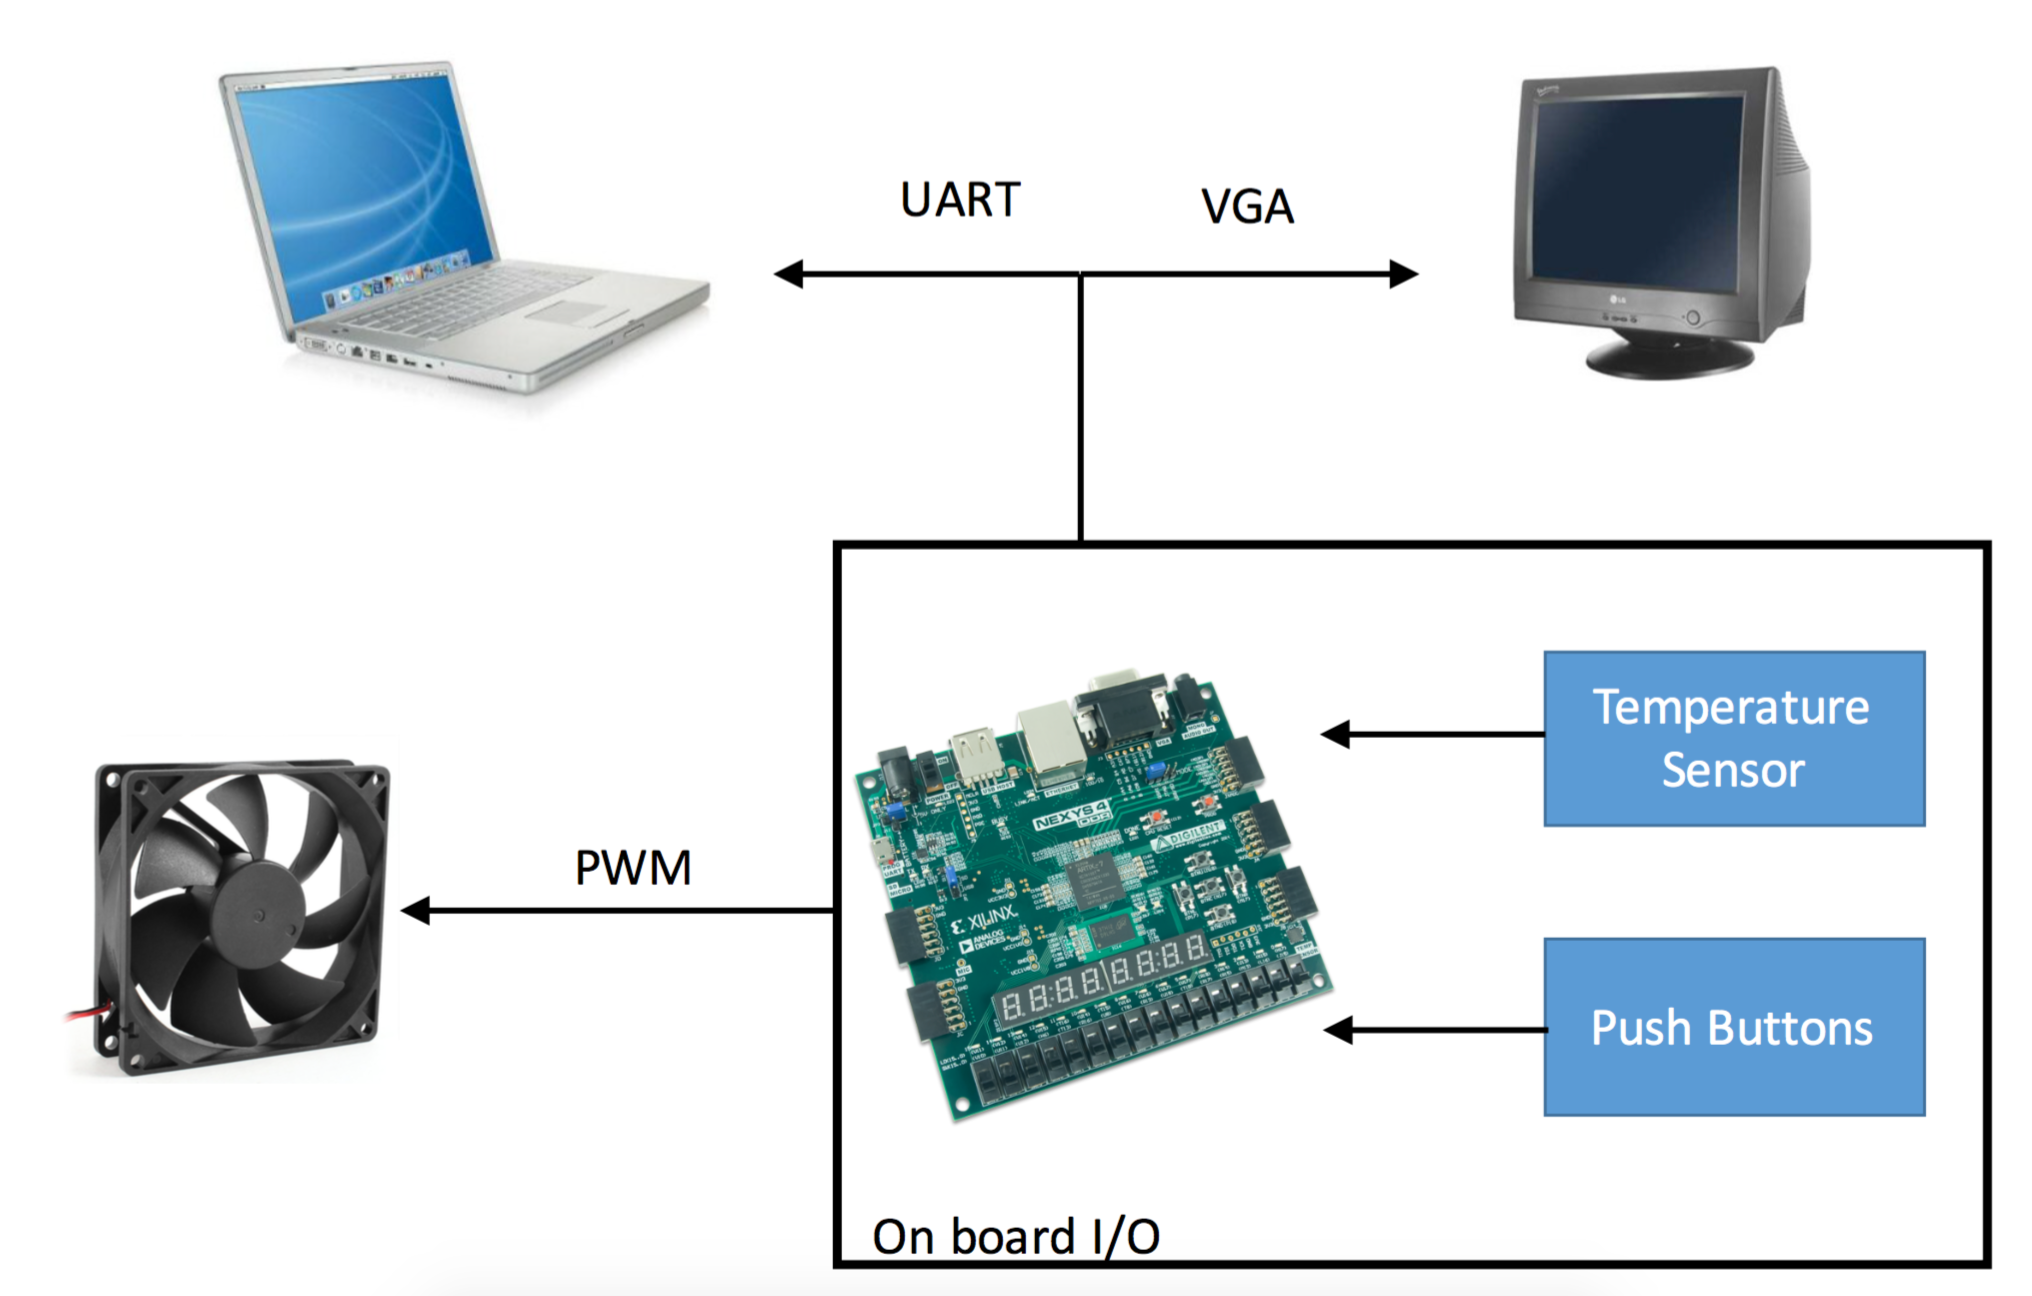
\includegraphics[scale=.4]{images/Overview}\\
\textbf{FIG 1.} High level overview of the system components.\\
\end{center}
\subsection{VHDL Project Overview}
Figure 2 shows an overview of the various VHDL components used in this project. The main modules that were developed for this project were $SetPointControl
$, $PIDController$, $TemperatureSensor$, $PWMInterface$, $Decimal2ASCII$ and $Values2Serial$. The remaining components were orignally written for use in other labs but were reused here. The only entity not developed in this course was the $UART$ component. This library was found online in order to speed up the the development of serial data capture, the original source can be seen in [1]. The three highest level components were instantiated in the top level coponents $TemperatureControlProject$.
\begin{center}
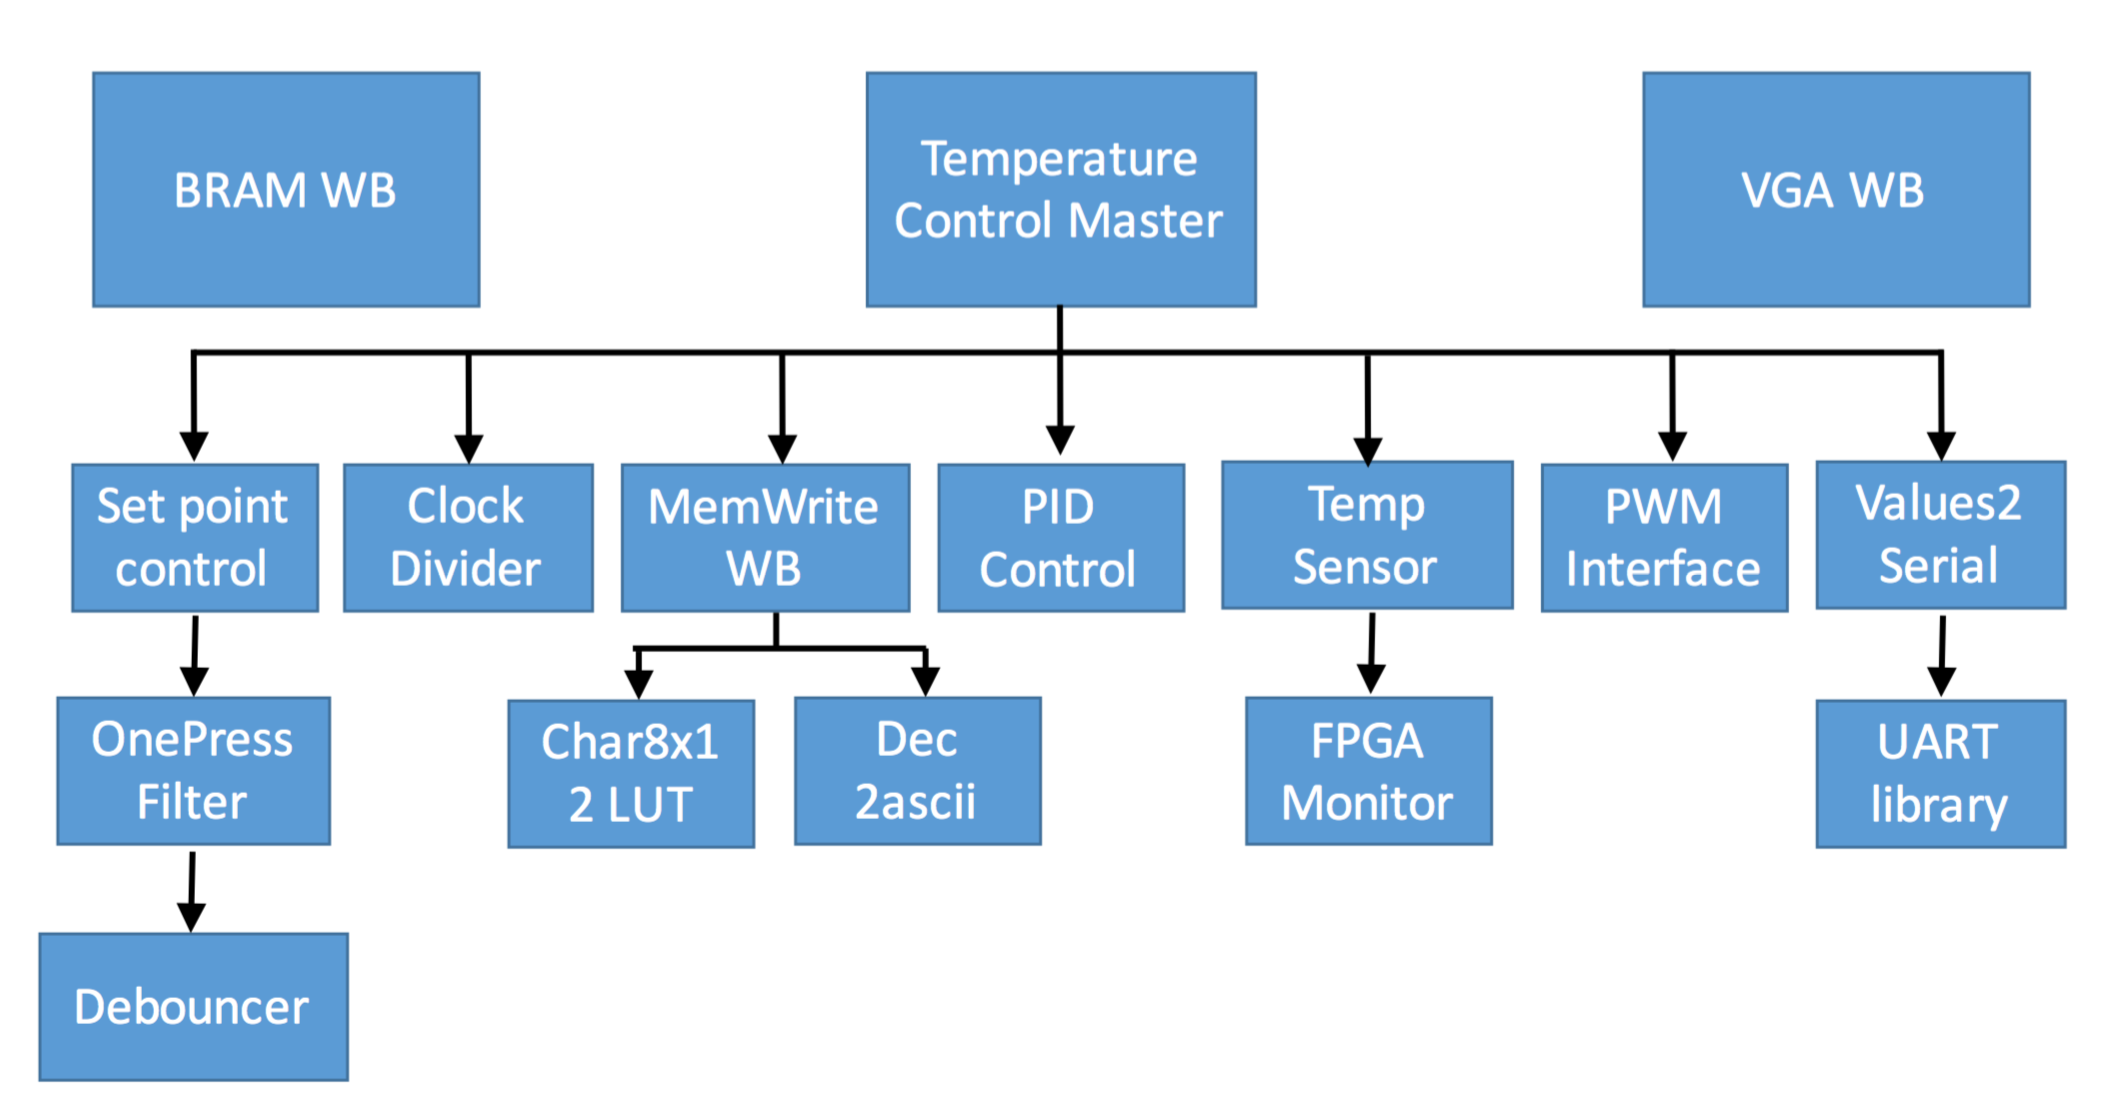
\includegraphics[scale=.35]{images/vhdl_arch}\\
\textbf{FIG 2.} High level VHDL component hierarchy.\\
\end{center}
 
\begin{center}
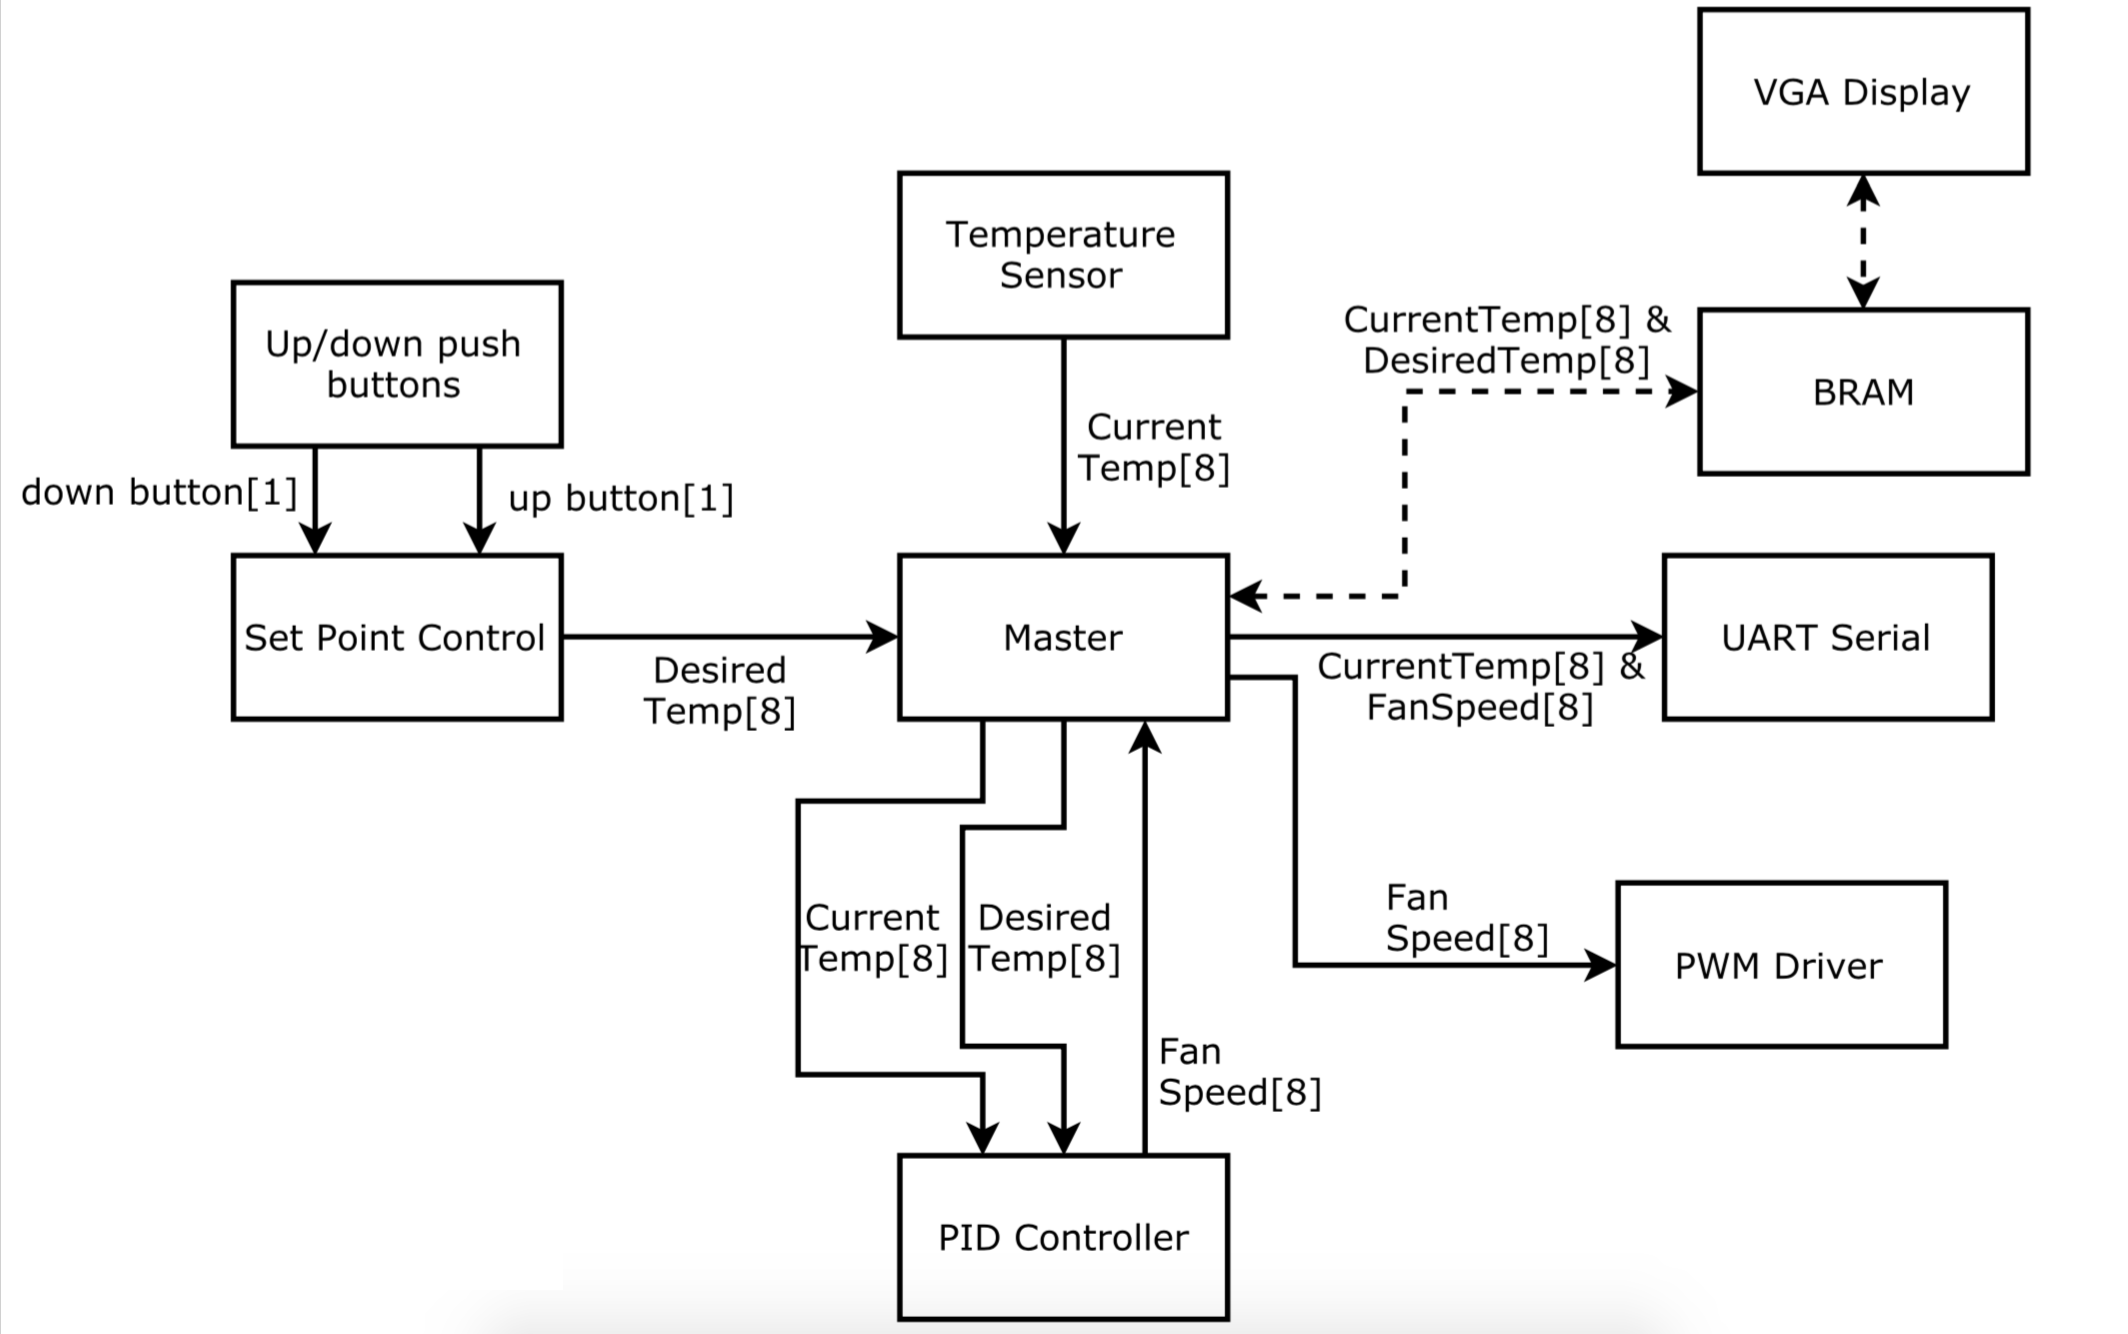
\includegraphics[scale=.4]{images/internalFlow}\\
\textbf{FIG 3.} Main component data path (Wishbone signals are shown as dotted lines).\\
\end{center}

Figure 3 shows the data path of the main components. The $Master$ component contains instantiations of $SetPointControl$, $PIDController$, $PWMDriver$, $TemperatureSensor$ and $UARTSerial$. I decided against making these specific components communicate over the wishbone bus due to the uncetain data send/retrival time that is introduced when communicating over a central bus. Because digital PID control must be normalized over a constant sampling rate, introducing unknown wait cycles did not seem like a good design choice. It may seem odd that I have the VGA controller communicating over the Wishbone bus but not the UART serial communication. This is because during development I was using the serial connection to collect data for the use of system identification and, once again, I did not want to introduce any unnesessary uncertainites into the data. Because the VGA display is just for the user, and is not a system critical component, any delays introduced by the bus wouldn't be an issue. 

\section{Temperature Sensor Module}
The temperature sensor used was included on the FPGA development board. The sensor is phycially located on the FPGA. Xilinx provided documentation on how to read and interpret the data from the sensor [2]. Xilinx also provided a VHDL module, $FPGAMonitor$, for returning the ADC(analog-digital converter) code from the on board temperature sensor. The ADC code then needs to be transformed to a meaningful temperature unit, in this project celcius is used. The equation for transforming the ADC code to a temperature is
\begin{align*}
Temp(\degree C) &= \frac{(ADCode)503.975}{4096}-273.15
\end{align*}
Derived from
\begin{align*}
Voltage &= 10\frac{kT}{q}ln(10)
\end{align*}
Where $k$ is Boltzmann's constant, $T$ is temperature in kelvin and q is the charge on an electron. The analog voltage is sampled by the 12-bit ADCX to produce an ADC code.
 This equation is implemented in the $TemperatureSensorModule$ component. The ADC code is returned in a 12-bit signal, 8-bits for integer values and 4 for decimal. For the sake of simplicity, I will only be using the 8-bits for integer values, which means the accuracy is in $1 \degree$C increments.
\begin{center}
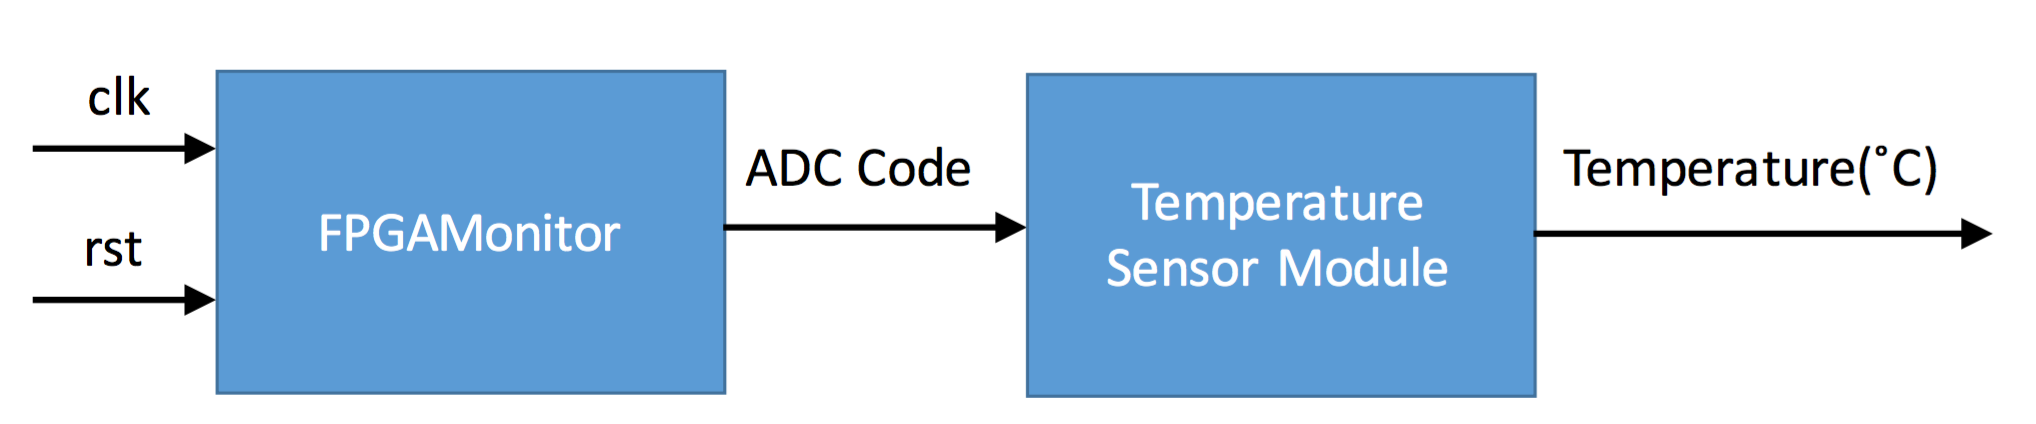
\includegraphics[scale=.4]{images/sensorM}\\
\textbf{FIG 4.} Block diagram of decoding sensor data.\\
\end{center}
\section{Desired Temperature Control Module}
To change the desired temperature during operation two push buttons are used. These buttons are bult into the FPGA development board. When pressed, the up button (BTNU) incrementes the desired temperature and the down button (BTND) decremements the desired temperature. To prevent mechanical glitches and make sure only one change is made per button press, a debouncer and one press filter were used. The state machine for the one press filter can be seen in figure 7. A button press event occurs only in the $press$ state. The $OnePressFilter$ VHDL module contains the button debouncer module. Two instantiations of the $OnePressFilter$ module are made in the $Master$ module. This module outputs a single 8-bit signal, containing the desired temperature.
\begin{center}
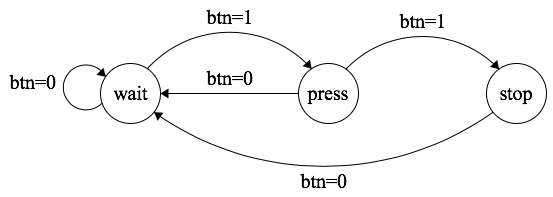
\includegraphics[scale=.5]{images/nopressMachine}\\
\textbf{FIG 5.} State machine diagram of the one press filter.\\
\end{center}
\section{DC Motor Control Module}
To alter the temperature of the FPGA, an off-the-shelf DC computer fan is used. To control the speed of the DC motor the FPGA outputs a PWM signal from the JA PMOD GPIO header. This module takes one 8-bit input signal containing the fan speed, which is limited to an integer with the range of 0 to 100. This value represents the fan speed from 0\% to 100\%. This value is then converted to a duty cycle percent using the logic shown in figure 6.
\begin{center}
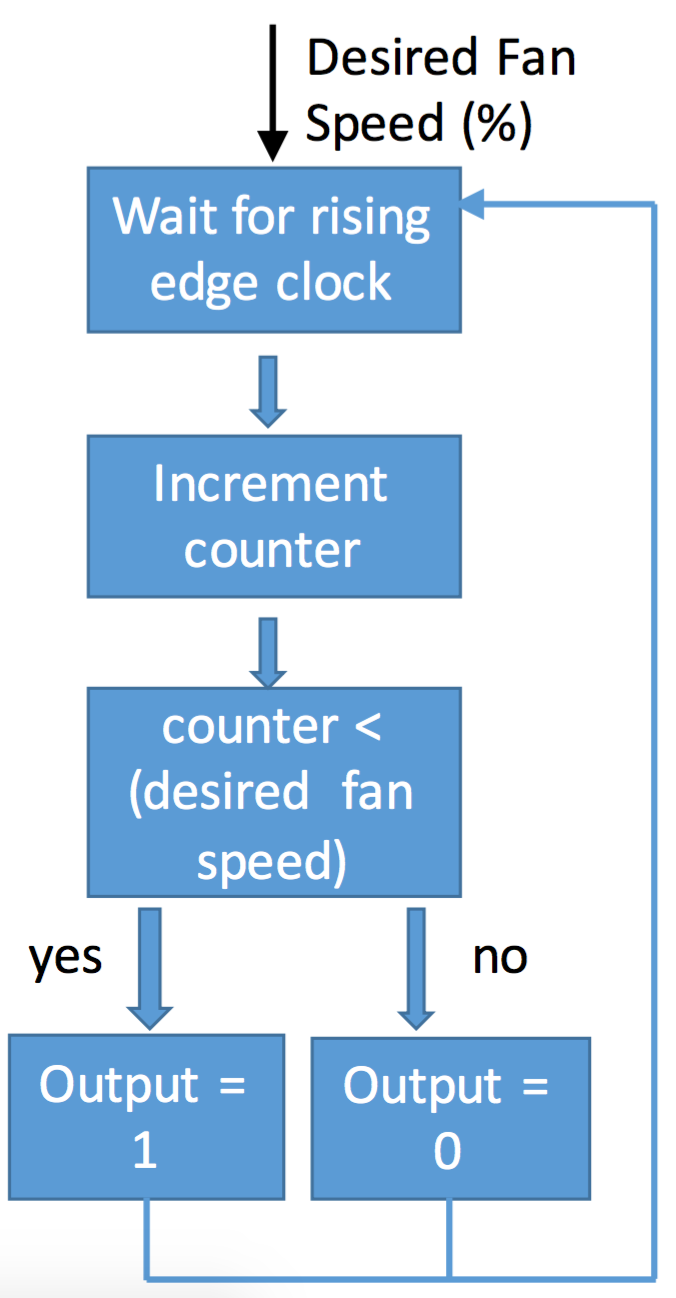
\includegraphics[scale=.4]{images/dutyPWM}\\
\textbf{FIG 6.} Duty cycle(\%) to PWM signal.\\
\end{center}

The FPGA PMOD output is a 0V LOW and 3.3V HIGH signal. However, the DC fan being used requires a potential of 5V. The 3.3V to 5V DC PWM motor driver circuit, shown in figure 7, was used to drive the fan. The circuit uses an n-MOSFET with a low threshold voltage. Specifically, the IRLB721 [3] was used due to its low max threshold voltage ($V_{TH_{max}}=2.35$V). The FPGA was more than adequetly able to switch the FET.

\begin{center}
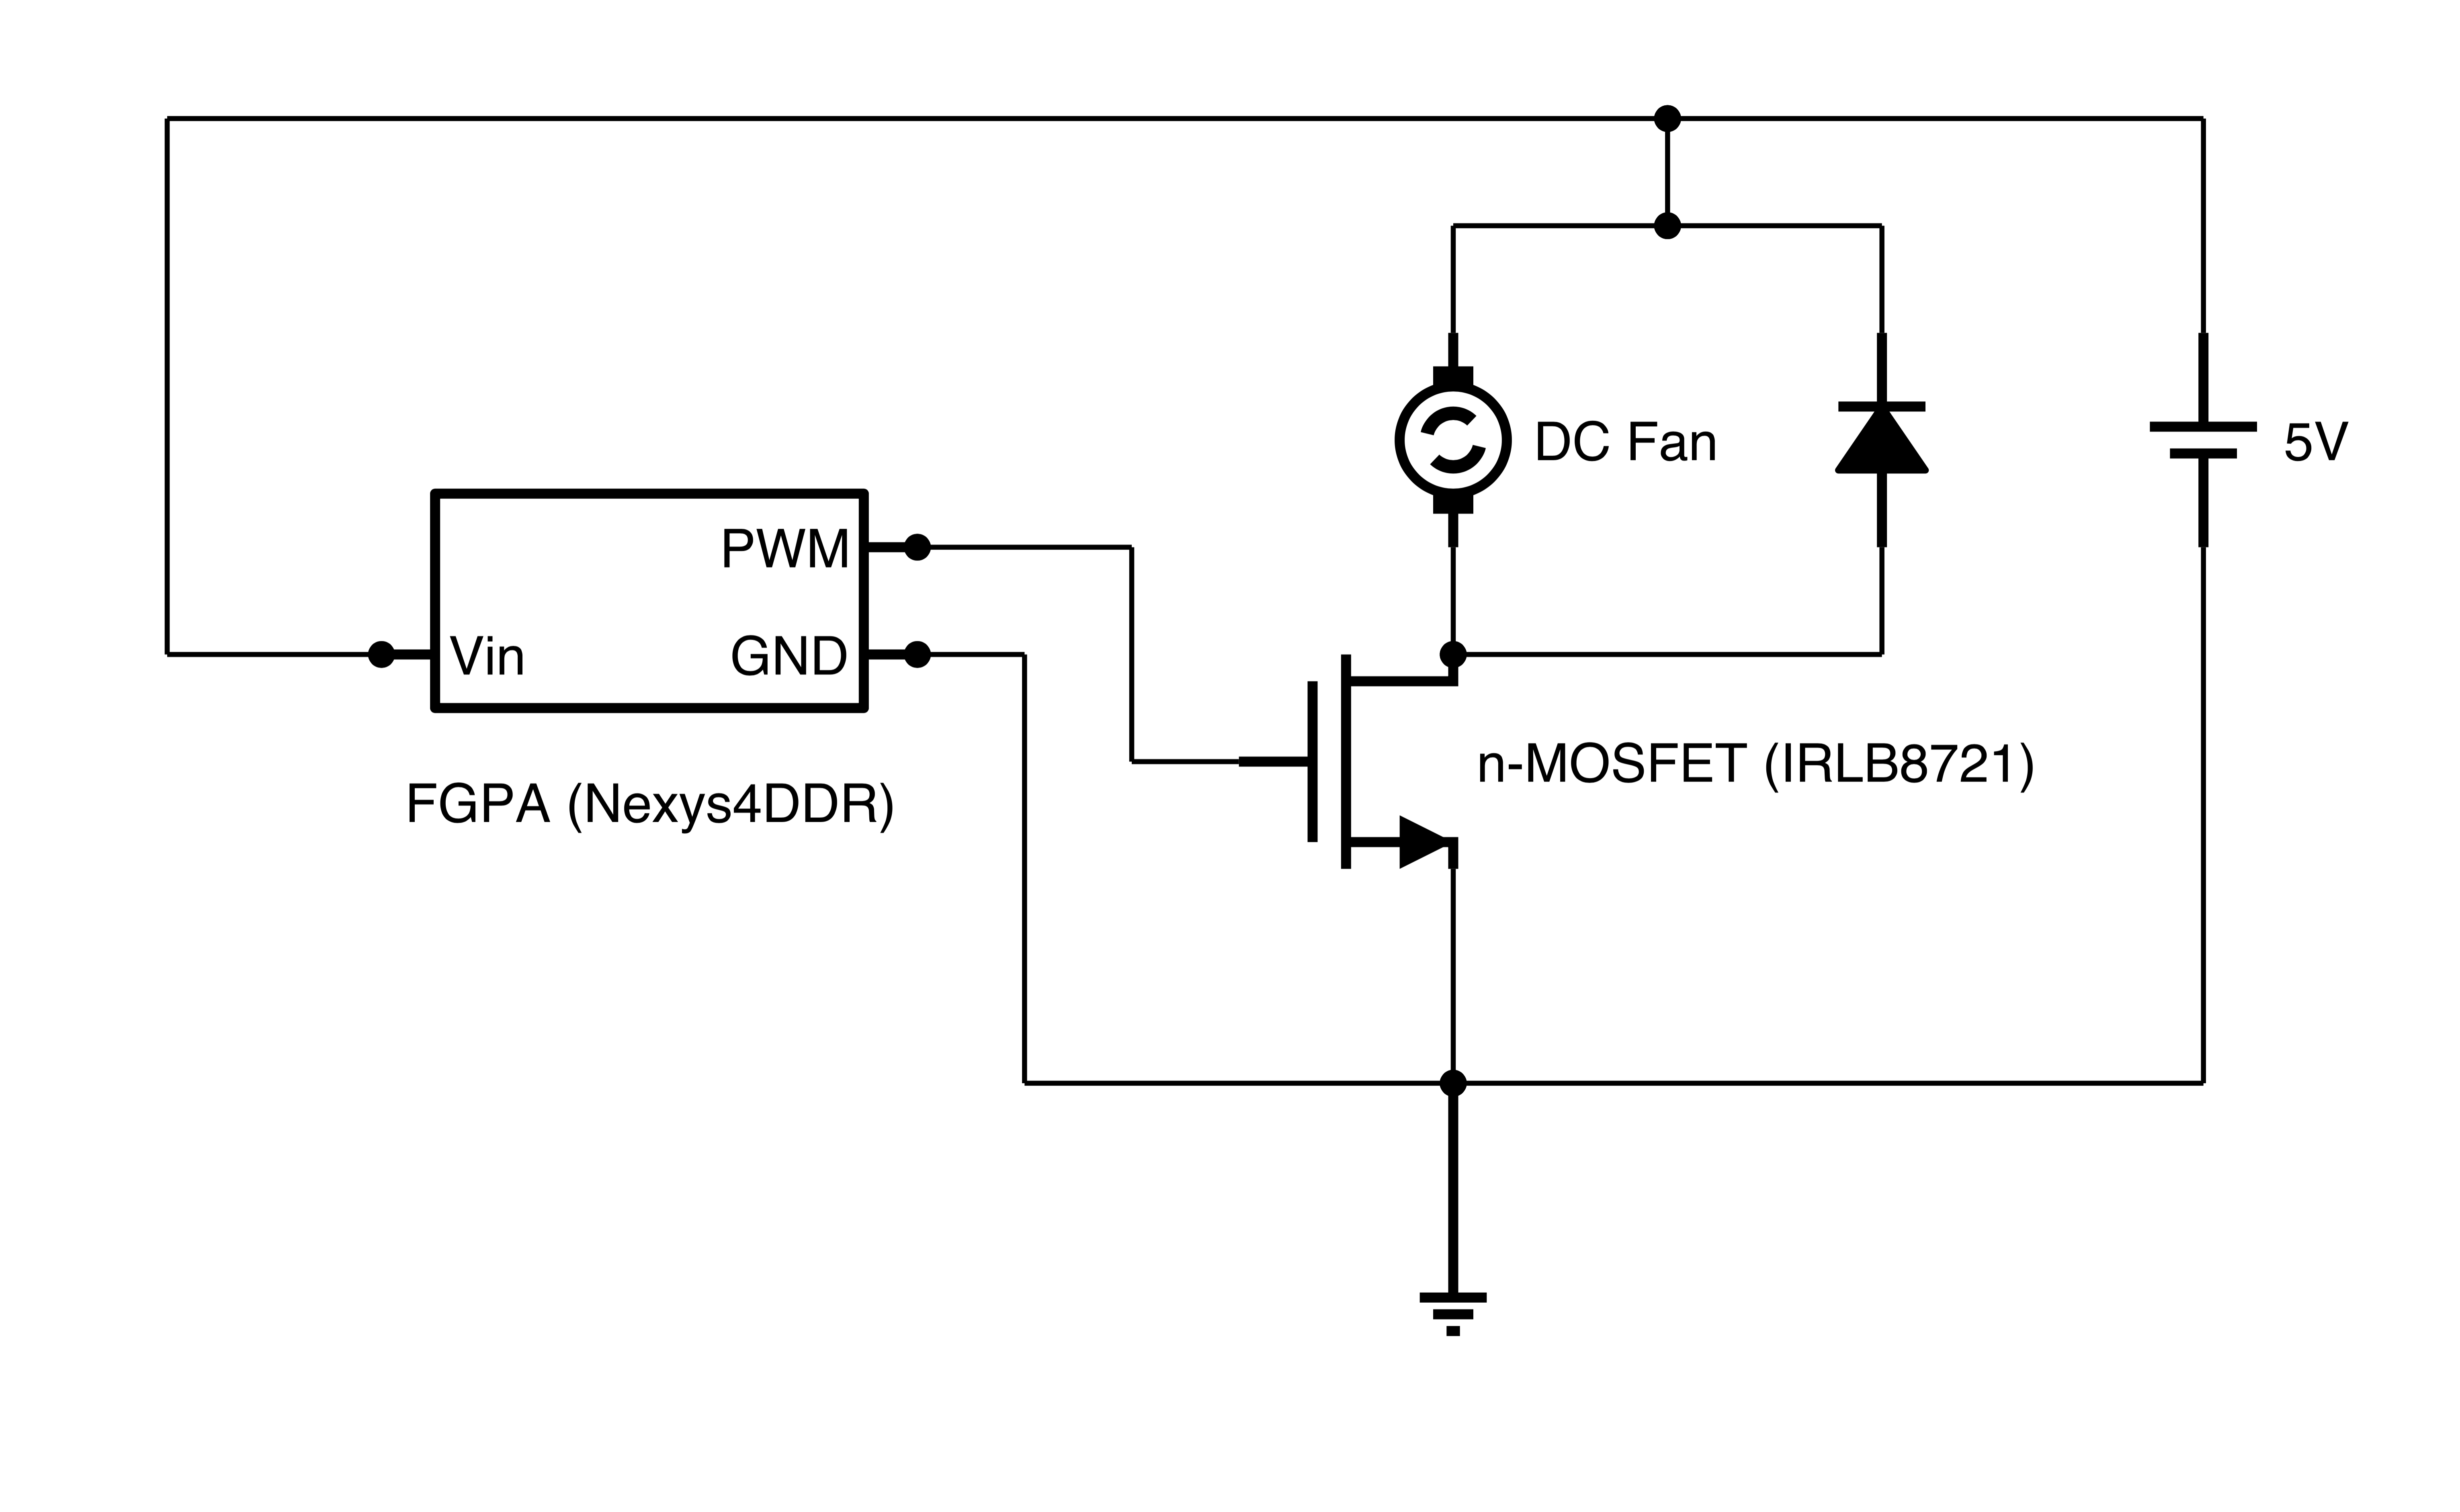
\includegraphics[scale=.5]{images/pwmSchematic-nowords}\\
\textbf{FIG 7.} 3.3V to 5V DC PWM Motor Driver Schematic.\\
\end{center}
\section{UART Serial Communication Module}
\subsection{UART Library Introduction}
For data aquisition I used a UART serial communication between the FPGA and an external computer. However, because this was not the main focus of this project I decided to find a library to simplify UART data transmission. I found a well documented library with plenty of usefull examples here [1]. However, to interface with this library another module needed to be created. The $Values2Serial$ module handles interfacing with the UART library. The UART library was contained in a single component and the I/O diagram can be seen in figure 8.
\begin{center} 
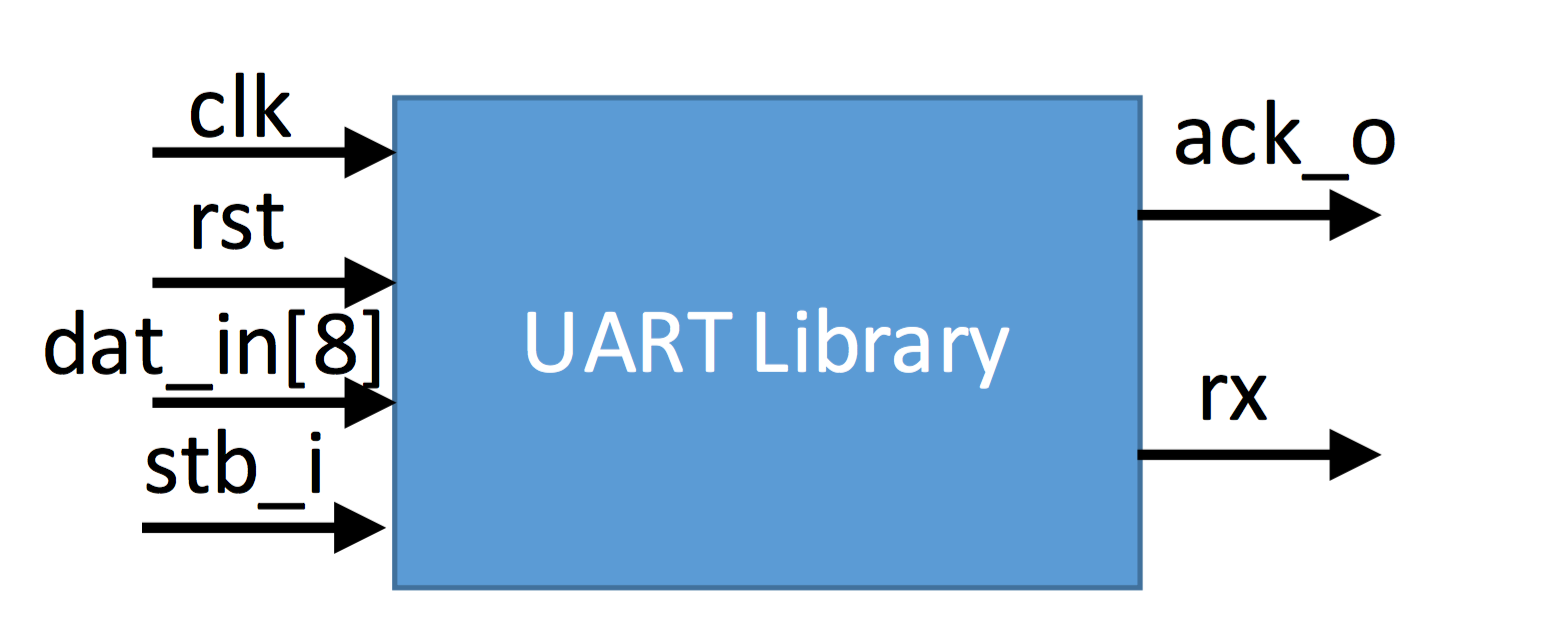
\includegraphics[scale=.4]{images/uartIO}\\
\textbf{FIG 8.} UART library component port map diagram (only relevent ports are shown).\\
\end{center}
Using this library did cause some issues during development. The hardware that the library was developed on used an active high reset scheme, which is opposite from the Nexys 4 DDR, so this caused some minor issues. Another variation was the TX/RX convention used by Xilinx differed from this library. Xilinx uses RX and TX from the perspective of the attatched device, in our case this would be the computer. So, the TX port is actually the port where the FPGA recieves data and the RX data is the port that the FPGA sends data. This was confusing to work through, but it was well documented in [2].
\begin{center}
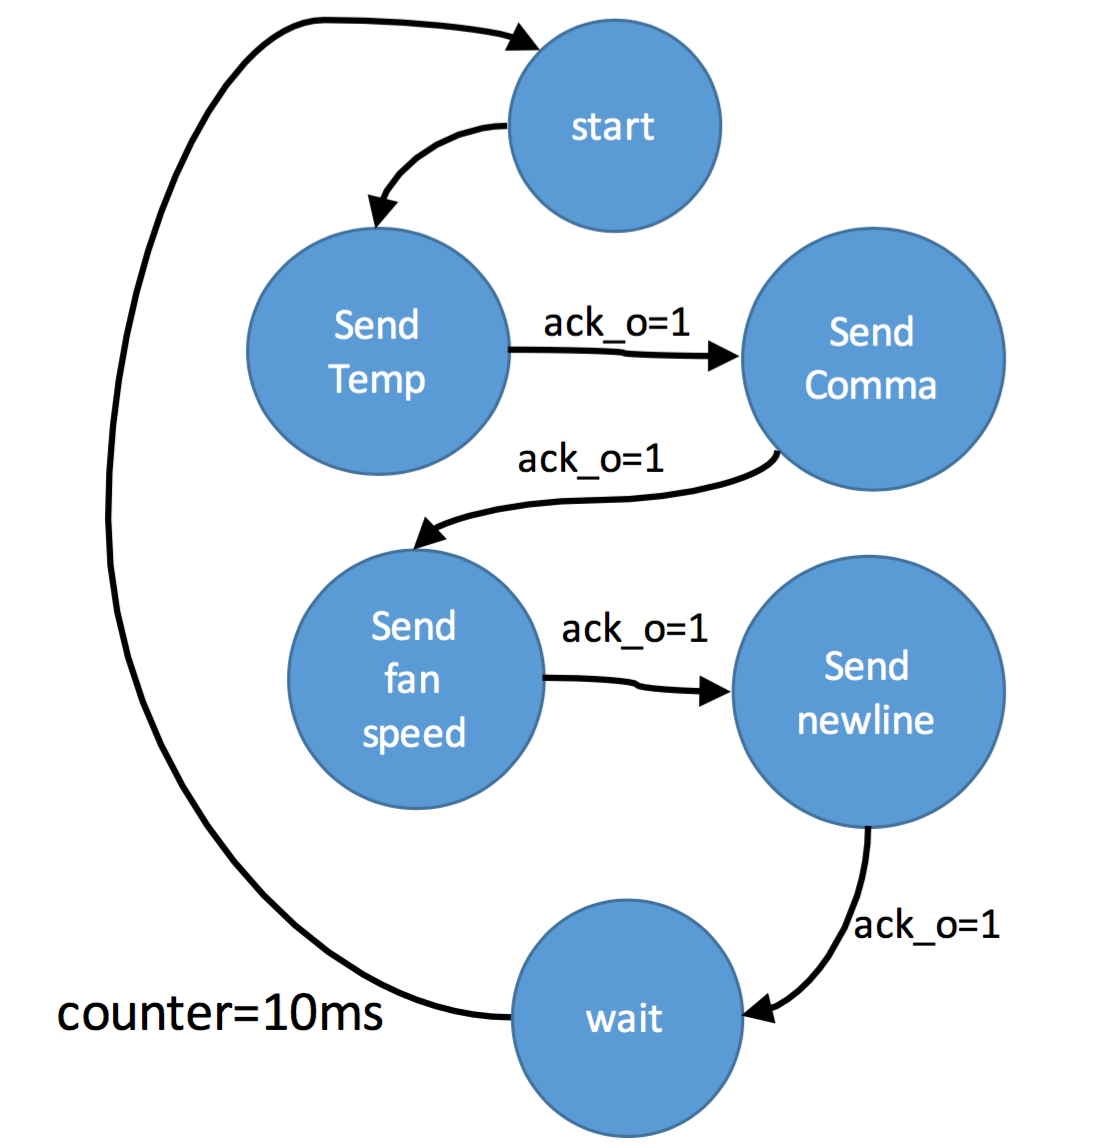
\includegraphics[scale=.35]{images/uartState}\\
\textbf{FIG 7.} 3.3V to 5V DC PWM Motor Driver Schematic.\\
\end{center}
\subsection{Using the UART Component}
The state machine shown in figure 9 describes how the $Values2Serial$ component interfaces with the UART library. The $UART$ component accepts 8-bit signals, so in order to send a message containing all the required data, a data transmission format was specified. To begin data transfer, the $stb\_i$ pin must be asserted and the data must be placed on the 8-bit $data\_in$ port. We must then wait for the $ack\_o$ to be asserted. When the $ack\_o$ is asserted, we deassert the $stb\_i$ pin and then wait for 10 ms, then repeat the process for the next 8-bit piece of data. 
\subsection{Data Encoding}
	To configure the connection on the external computer any standard serial communication software can be used. Howver, the settings must be confgured to the following settings: baud rate=115200, data bits=8, parity=none, stop bits=1. The data being recieved will be in the follwing format: XX2CXX0A. Where the XX represents an 8-bit hexidecimal number, and 2C is the hexidecimal representation of the ASCII comma (,) character and 0A is the hexidecimal representation of the ASCII newline character ($\backslash$n). The first XX contains the current temperature and the second XX contains the current fan speed. Below is an example of the raw serial output. 

\begin{center}
	24 2C 17 0A 24 2C 17 0A 23 2C 17 0A 23 2C 17 0A 22 2C 17 0A 22 2C 17 0A\\
\end{center}
To decode this we start reading it left to right. We first see the hexidecimal 62, if we reference our data format from above, we see that this first number is our current temperature in hexadecimal. For it to be human readable we must convert it to decimal, 0x24 => 36. So, the current temperature is $36\degree$C. Moving to the next number we see 2C, again we reference our data format from above and see that this is just ASCII for a comma (,). The next number is hexadecimal 17. Check the format guide and decode to decimal, we can see that this shows the fan speed is 23$\%$. The next number is 0A, which is ASCII for a newline character. This concludes one data reading from the FPGA. Repeat the above procedure to decode the entire message. However, that doesn't seem like very much fun. So, I wrote the below Python script to automate the data interpretation.

\begin{lstlisting}
f = open('dataFromSerial.txt')
file = open('decodedData.txt', 'w')
data = f.readline().split("0A")
for line in iter(data):
	d = line.split("2C")
	try:
		x = str(int(d[0],16))+ ", " + str(int(d[1],16))
		print(x)
		file.write(x+'\n')
	except ValueError:
		print("there was probably a problem or something")
f.close()
file.close()
\end{lstlisting}
If we pass the above data stream to this Python function we get the following as output in much easier to read format (Current temperature, fan speed).
\begin{center}
36, 23\\
36, 23\\
35, 23\\
35, 23\\
34, 23\\
34, 23\\
\end{center}

\section{VGA BRAM Display Module}
\section{Digital PID Control Module}
\subsection{Discrete PID Control Background}
\begin{align*}
e[k] &= r[k]-y[k]\\
f[k+1] &= K_pe[k]+K_i\sum e[k]T_s + K_d\dfrac{e[k]-e[k-1]}{T_s}\\
T_s&=0.01 s
\end{align*}
The below code sample is the VHDL implementation of the discrete PID controller shown in the equations above.
\begin{lstlisting}
elsif(samplingRateClock'event and samplingRateClock='1') then
			error := (setpoint - sensorFeedbackValue); --compute new error e[k]
			errorSum	:= errorSum + error; --continually compute discrete integral
			if(errorSum > 10000) then --integral wind up check
				errorSum := 10000;
			elsif(errorSum < -10000) then
				errorSum := -10000;
			end if;
			errorChange := error - previousError; --compute discrete derivative
			output := (kp*error + ki*errorSum + kd*errorChange)/100; --compute and scale output
			previousError := error; --save error for use in next iteration for discrete derivative
			if(output>100) then --saturate sensor if needed
				output := 100;
			elsif(output<0)then
				output:=0;
			end if;
			controllerOutput<= output;
	end if;
\end{lstlisting}
\subsection{System Identification}
 \begin{align*}
\boldsymbol{x}[k+1] &= \boldsymbol{A}\boldsymbol{x}[k] + \boldsymbol{B}(\delta[k]-f[k])\\
\boldsymbol{y}[k] &= \boldsymbol{C}\boldsymbol{x}[k]
\end{align*}
\begin{align*}
  \boldsymbol{x}[k+1] &= \begin{bmatrix}
	1 & 0.001 & 0 & 0\\
	0 & 1 & -0.00196 & 0\\
	0 & 0 & 1 &0.001 \\
	0 & 0 & 0.02352 & 1
\end{bmatrix}\boldsymbol{x}[k]+\begin{bmatrix} 0 \\ 0.002 \\ 0 \\ -0.004\end{bmatrix}u[k]\\\\
\boldsymbol{y}[k] &= \begin{bmatrix}
	1 & 0 & 0 & 0\\
	0 & 0 & 1 & 0\\
\end{bmatrix}\boldsymbol{x}[k]
\end{align*}
\subsection{Digital PID Control System Design}
\begin{center}
$K_p=545$	$K_i=150$	$K_d=22$
\end{center}
\section{Implementation Images}

\section{References}

[1] \url{http://bytebash.com/2011/10/rs232-uart-vhdl} \newline
[2] \url{http://www.xilinx.com/support/documentation/user_guides/ug480_7Series_XADC.pdf}, page 23 \newline
[3] \url{https://www.adafruit.com/products/355}

\section{Appendix}
1. VHDL implementation of main components.
\end{document}

